\chapter{Indledning}

\section{Baggrund}
I Danmark er den demografiske udvikling under stor vækst. Denne skaber en række demografiske sårbarheder, som regeringen, religioneren og kommunerne ikke kan undgå at reagere på. KL har i 2014 lavet en analyserapport "Danmark i forandring", der gennem statistikker fra Danmarks statistik klarlægger forskellige tendenser. I rapporten er der forskellige fremskrivninger, der bygger på gennemsnittet af en række fremskrivningsparametre over de foregående fire år (fra 2010-2014)\footnote{Analyserapport KL}. Fremskrivninger er dermed ikke en prognose, men et billede for, hvordan fremtiden vil se ud, hvis de samme tendenser foreligger. Første kapitel tager fat i befolkningsudviklingen og den demografiske udvikling. \\
Konklusionen er, at kommuner udenfor de store byer er præget af flere ældre, færre erhvervsaktive og lave fødselstal. Fra 1980 til 2014 er der blevet knap 10 pct. flere borger i Danmark. Tendensen er, at flere og flere flytter fra yderkommunerne til bykommunerne\footnote{Analyserapport KL figur 1.1 og 1.2 }. Tallene viser at gennemsnitsalderen er voksende. Den er steget med 4 pct. fra 1980 til 2014. Yderkommunerne har den højste gennemsnitsalder, mens bykommunerne scorer den laveste\footnote{Analyserapport KL figur 1.6}. Disse tendenser påvirker ældrekvoten, som er en af de store udfordringer. Udviklingen gør, at der er færre personer i den arbejdsdygtige aldre til at forsørge de flere udenfor denne aldre\footnote{Analyserapport KL tabel 1.1, figur 1.8}.

\begin{figure}[H]
\centering
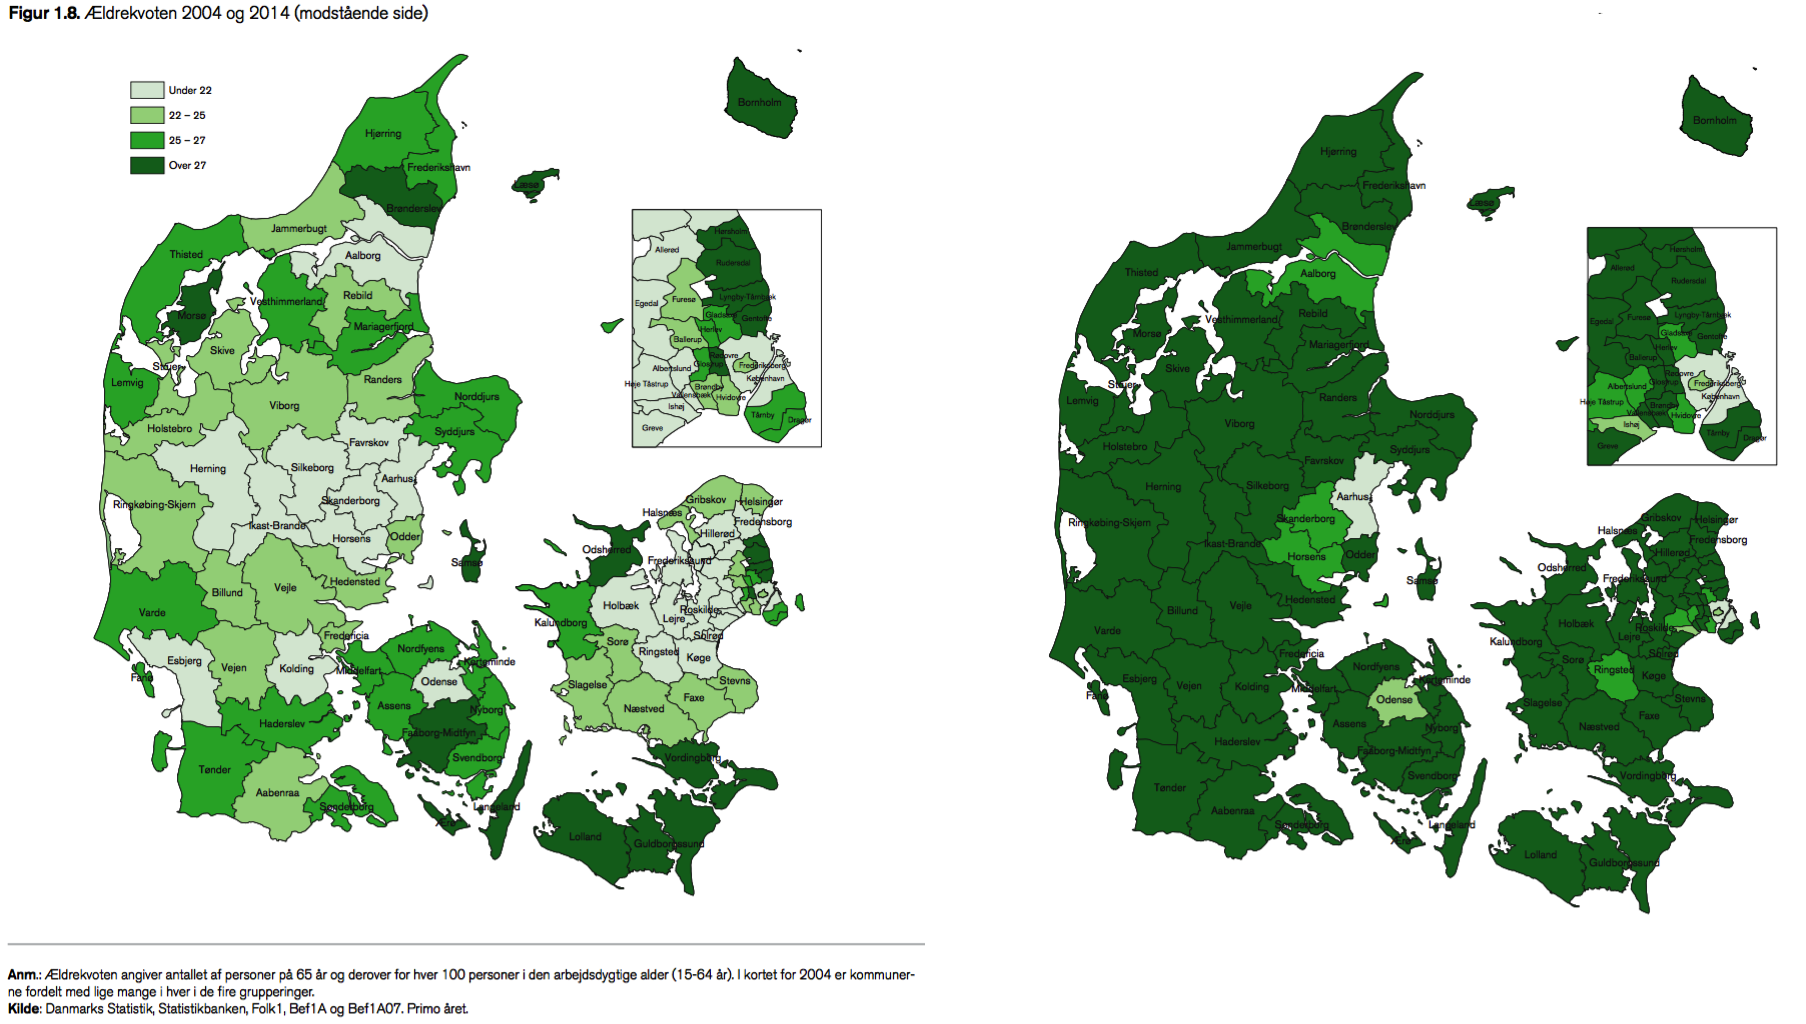
\includegraphics[width=1\textwidth]{Figurer/Snip20160428_14}
\caption{Figur 1.8 fra "Kommunernes strategi for telesundhed". Ældrekvoten i Danmark fra 2004 (venstre) og fra 2014 (højre)}
	
\end{figure}

 Dette vil på sigt skabe store problemer, særligt indenfor sundheds- og plejesektoren både samfundsøkonomisk og ressourcermæssigt. Der vil være færre til at betale skat, hvilket resulterer i, at det at forsørge de ældre vil blive dyrere og dyrere for samfundet. 
Med disse demografiske samt økonomiske udfordringer Danmark står overfor, er det nødvendigt at tænke i andre baner. Sundhed skal leveres på nye mere smarte og teknologiske måder.        

Telemedicin er derfor for alvor kommet på dagsorden hos regeringen, religionerne og kommunerne. I 2012 udarbejdede disse parter en ambitiøs national handlingsplan for udbredelsen af telemedicin i Danmark\footnote{\url{http://www.digst.dk/Digital-velfaerd/Initiativer-og-projekter/Projekter-i-Strategi-for-digital-velfaerd/Udbredelse-af-telemedicin-i-hele-landet_fokusomraade1} - Besøg d. 28-04-2016 - Opdateret d. 28-01-2016}. Arbejdet med denne handleplan skal give den vigtige erfaring med telemedicin samt give mulighed for parterne at udarbejde fælles modeller for samarbejde, arbejdsgange, økonomiske konsekvenser og øvrige effekter af de konkrete telemedicinske løsninger. Et af de helt klare formål med denne handleplan, er at sikre, at udbredelsen af telemedicin til nye patientgrupper og behandlingsområder vil forløbe hurtigere og mere sikkert i fremtiden. Målet er også at skabe fælles nationale standarder for sundheds-it, så nye telemedicinske løsninger udvikles, så systemerne kan arbejde sammen på tværs\footnote{Telemedicin en nøgle til fremtidens sundhedsydelser}. \\
Digitaliseringsstyrelsen ser også mulighederne for de telemedicinske løsninger og er ved at lave en ny fællesoffentlig digitaliseringsstrategi frem mod 2020, hvor et af pejlemærkerne tager udgangspunkt i den offentlige sektor digitalisering, og som har datadeling, datasikkerhed og it-infrastruktur som temaer \footnote{\url{http://www.digst.dk/Digitaliseringsstrategi/Ny-digitaliseringsstrategien-2016-2020/Kommissorium-og-maalbillede-2020} - Besøgt d. 28-04-2016 - Opdateret d. 25-04-2016}. Denne strategi skal understøtte de teknologiske muligheder for smartere og mere sikker deling af data mellem borger og offentlige sektor\footnote{målbillede for strategi for digitaliseringen}.\\
Kommunernes strategi er fokuseret bredere - nemlig på telesundhed og ikke telemedicin.

Telemedicin er en under begreb indenfor telesundhed, hvor telesundhed indgår i det overordnede begreb velfærdsteknologi\footnote{Kommunernes strategi for telesundhed}. Forholdet mellem de tre begreber er illustreret i figur 1.1. 

\begin{figure}[H]
	\centering
	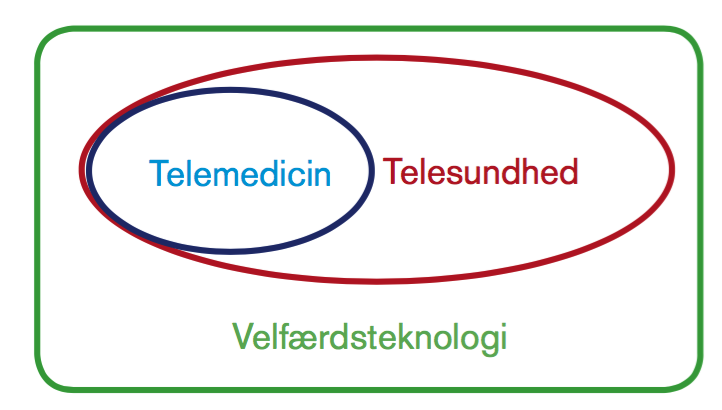
\includegraphics[width=0.8\textwidth]{Figurer/Snip20160426_6}
	\caption{Forholdet mellem velfærdsteknologi, telesundhed og telemedicin \protect\footnotemark}
\end{figure}
\footnotetext{Kommunernes strategi for telesundhed}

I "Kommunernes strategi for telesundhed"\ defineres telesundhed som brugen af informations- og kommunikationsteknologi til at understøtte, forebygge, behandlende eller rehabiliterende aktiviteter over afstand. Telesundhed tager udgangspunkt i borgeren og borgerens samlede behov for kontakt med sundhedsvæsenet. Derimod er telemedicin mere fokuseret på selve diagnosen og behandlingen borgeren har behov for. Telesundhed fokuserer på borgernes helbred inden, de bliver patienter\footnote{\url{http://sundhedsdatastyrelsen.dk/da/rammer-og-retningslinjer/om-digitaliseringsstrategi/telemedicin-og-telesundhed} - Besøgt d. 28-04-2016 - Opdateret d.16-02-2015 \& Kommunernes strategi for telesundhed}.

Kommunernes mål med telesundhed er at gøre borgerne mere selvstændige, uafhængige af tid og sted og øge deres følelsen af at kunne mestre eget liv. Gennem telesundhed skal de sundhedsprofessionelle kunne motivere borgerne i ændrede vaner som er sundhedsfremmende eller forebyggende. Det sidste og måske vigtige mål er, at telesundhed som minimum skal kunne levere ydelserne af samme kvalitet som før\footnote{Kommunernes strategi for telesundhed}. 

Det danske sundhedssystem står overfor store forandringer, hvor sygehusene bliver specialiseres og samles på færre og større enheder. Behandlingerne bliver mere skånsomme, da hurtig mobilisering af patienten reducerer indlæggelsestiden og en hurtigere rehabilitering, hvilket økonomisk set giver en stor gevinst. Denne udvikling vil give nye kommunale opgaver, som telesundhed med stor fordel kunne varetage     \footnote{Kommunernes strategi for telesundhed}.

Telesundhed dækker som tidligere nævnt meget bredt, og kommunerne ser et stort potentiale til flere forskellige opgaver. I hjemmeplejen har man i flere kommuner forsøgt sig med virtuel hjemmepleje, hvor påmindelse om medicin- og fødeindtage bliver kommunikeret over videokonference mellem borger og sundhedsprofessionelle. Viborg kommune har efter et pilotprojekt fra 2013 gode erfaringer med virtuel hjemmepleje og har fra 2014 til 2017 et  udviklings - og forskningsprojekt kørerende\footnote{\url{http://kommune.viborg.dk/Borger/Seniorer-og-pensionister/Hjaelp-i-hjemmet/Velfaerdsteknologi/Teknologier-og-projekter/Telesundhed/Virtuel-hjemme-og-sygepleje} - Besøgt d. 28-04-2016 - Opdateret d. 26-05-2015}. Halsnæs kommune har også i 2014 satset på virtuel hjemmepleje efter inspiration fra pilotprojektet fra Viborg kommune\footnote{Halsnæs virtuel hjemmepleje}.    
 

\section{Formål}
Denne mini-MTV har til formål at vurdere virtuel hjemmepleje i Favrskov kommune. Netplan Care og Favrskov Kommune er i gang med et innovationssamarbejde om udviklingen af en kommunal digital velfærdsteknologisk sundhedsstrategi for telesundhed. 
\\ \\
Telesundhed dækker over digitale velfærdsydelser på mobil- og bredbåndsnettet, hvor sundhedsfaglig dialog og behandling ved brug af den digitale infrastruktur muliggør, at borgere smidigt og omkostningseffektivt kan komme i kontakt med sundhedsvæsenet.    
\\ \\
Video er den mest komplekse løsningskomponent i forhold til telesundhedsløsninger. En af de digitale velfærdsteknologier Favrskov Kommune arbejder med at implementere er Virtuel hjemmepleje, som i høj grad benytter videos som et redskab til kommunikation mellem borger og sundhedsprofessionel. 
\\ \\
Sundhedsteknologistuderende fra Aarhus Ingeniørhøjskole udarbejder i samarbejde med Netplan Care og Favrskov Kommune en Medicinsk Teknologi Vurdering af videobaserede løsninger for Virtuel hjemmepleje. Analysen skal især afdække de teknologiske aspekter samt borgeres reaktioner på video som telesundhedsløsning. Ligeledes vil aspektet om organistionen være i fokus. 

\section{Fokuserede spørgsmål}
\begin{itemize}
	\item Hvilke forudsætninger skal der til for at video fungerer i telesundhedsløsninger? 
	\item Hvilket behov kan video i telesundhedsløsninger dække?
	\item Hvordan er brugernes reaktion og hvad skal man være opmærksom på, opdelt på de sundhedsprofessionelle og borgerne. 
\end{itemize}

